\documentclass[border=8pt]{standalone}
\usepackage{lmodern}
\usepackage{tikz}
\usepackage{amsmath,amssymb}
\usetikzlibrary{arrows.meta,positioning,calc}

\definecolor{kmblue}{HTML}{003874}
\definecolor{kmgold}{HTML}{BA9224}
\definecolor{rtpurple}{HTML}{7E22CE}
\definecolor{rtgreen}{HTML}{15803D}
\definecolor{rtred}{HTML}{DC2626}
\definecolor{axgray}{HTML}{94A3B8}
\definecolor{dkgray}{HTML}{334155}
\definecolor{ltbg}{HTML}{F8FAFC}

\begin{document}
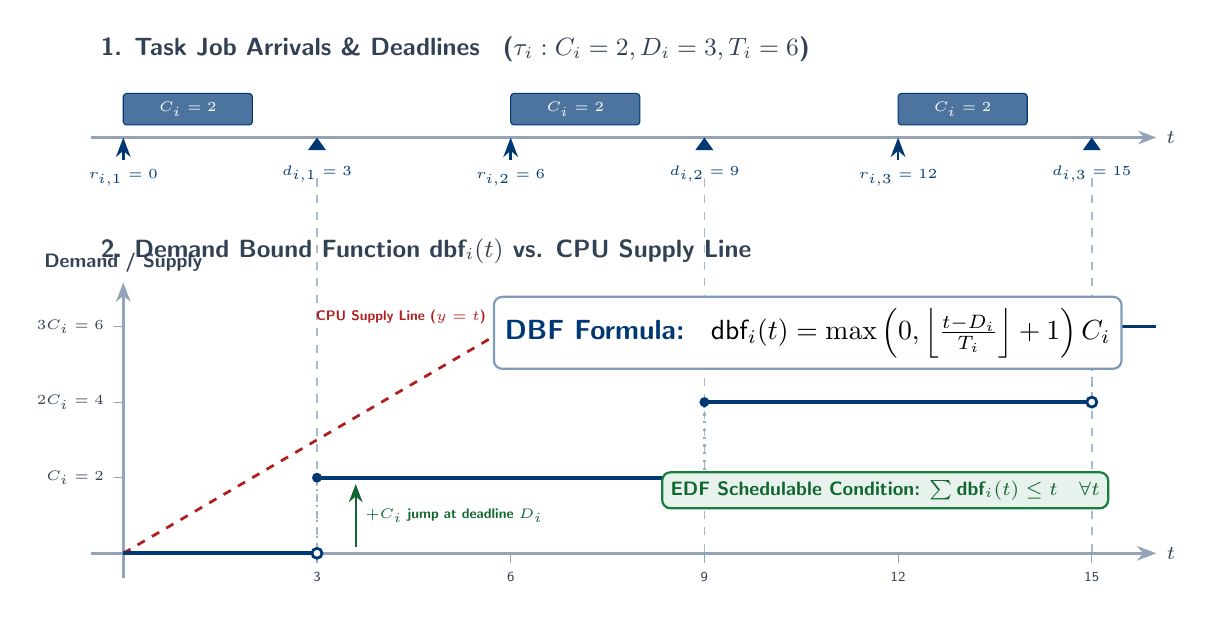
\begin{tikzpicture}[>=Stealth,font=\sffamily,x=0.82cm,y=0.80cm]

  % =====================================================================
  % TOP PANEL: Task Job Arrivals & Deadlines
  % Task tau_i = (C_i=2, D_i=3, T_i=6)
  % =====================================================================
  \def\yT{6.6}

  % Panel Header
  \node[dkgray,font=\sffamily\small\bfseries,anchor=west] at (-0.5, 8.0)
        {1. Task Job Arrivals \& Deadlines \enspace ($\tau_i: C_i=2, D_i=3, T_i=6$)};

  % Time Axis Top
  \draw[axgray,line width=0.8pt,->] (-0.5, \yT) -- (16.0, \yT)
        node[right,font=\sffamily\scriptsize\bfseries,dkgray] {$t$};

  % Job 1: Release 0, Deadline 3, Execution [0,2]
  \fill[kmblue!70,rounded corners=1.2pt] (0, \yT+0.2) rectangle (2, \yT+0.7);
  \draw[kmblue,line width=0.4pt,rounded corners=1.2pt] (0, \yT+0.2) rectangle (2, \yT+0.7);
  \node[white,font=\sffamily\tiny\bfseries] at (1, \yT+0.45) {$C_i=2$};
  \draw[kmblue,line width=0.9pt,->] (0, \yT-0.35) -- (0, \yT) node[pos=0,below,font=\sffamily\tiny\bfseries] {$r_{i,1}=0$};
  \fill[kmblue] (3, \yT) -- (2.86, \yT-0.2) -- (3.14, \yT-0.2) -- cycle;
  \node[kmblue,font=\sffamily\tiny\bfseries,below=2pt] at (3, \yT-0.2) {$d_{i,1}=3$};

  % Job 2: Release 6, Deadline 9, Execution [6,8]
  \fill[kmblue!70,rounded corners=1.2pt] (6, \yT+0.2) rectangle (8, \yT+0.7);
  \draw[kmblue,line width=0.4pt,rounded corners=1.2pt] (6, \yT+0.2) rectangle (8, \yT+0.7);
  \node[white,font=\sffamily\tiny\bfseries] at (7, \yT+0.45) {$C_i=2$};
  \draw[kmblue,line width=0.9pt,->] (6, \yT-0.35) -- (6, \yT) node[pos=0,below,font=\sffamily\tiny\bfseries] {$r_{i,2}=6$};
  \fill[kmblue] (9, \yT) -- (8.86, \yT-0.2) -- (9.14, \yT-0.2) -- cycle;
  \node[kmblue,font=\sffamily\tiny\bfseries,below=2pt] at (9, \yT-0.2) {$d_{i,2}=9$};

  % Job 3: Release 12, Deadline 15, Execution [12,14]
  \fill[kmblue!70,rounded corners=1.2pt] (12, \yT+0.2) rectangle (14, \yT+0.7);
  \draw[kmblue,line width=0.4pt,rounded corners=1.2pt] (12, \yT+0.2) rectangle (14, \yT+0.7);
  \node[white,font=\sffamily\tiny\bfseries] at (13, \yT+0.45) {$C_i=2$};
  \draw[kmblue,line width=0.9pt,->] (12, \yT-0.35) -- (12, \yT) node[pos=0,below,font=\sffamily\tiny\bfseries] {$r_{i,3}=12$};
  \fill[kmblue] (15, \yT) -- (14.86, \yT-0.2) -- (15.14, \yT-0.2) -- cycle;
  \node[kmblue,font=\sffamily\tiny\bfseries,below=2pt] at (15, \yT-0.2) {$d_{i,3}=15$};

  % Vertical projection lines linking deadlines to staircase steps
  \foreach \t in {3,9,15} {
    \draw[kmblue!35,line width=0.6pt,dashed] (\t, \yT-0.65) -- (\t, 0.0);
  }

  % =====================================================================
  % BOTTOM PANEL: Demand Bound Function dbf_i(t) Curve
  % =====================================================================

  % Panel Header
  \node[dkgray,font=\sffamily\small\bfseries,anchor=west] at (-0.5, 4.8)
        {2. Demand Bound Function $\text{dbf}_i(t)$ vs. CPU Supply Line};

  % Axes
  \draw[axgray,line width=0.9pt,->] (-0.5, 0) -- (16.0, 0)
        node[right,font=\sffamily\scriptsize\bfseries,dkgray] {$t$};
  \draw[axgray,line width=0.9pt,->] (0, -0.4) -- (0, 4.3)
        node[above,font=\sffamily\scriptsize\bfseries,dkgray] {Demand / Supply};

  % Ticks on x-axis
  \foreach \t in {3,6,9,12,15} {
    \draw[axgray] (\t, 0) -- (\t, -0.15)
          node[below,font=\sffamily\tiny,dkgray] {\t};
  }

  % Ticks on y-axis
  \draw[axgray] (0, 1.2) -- (-0.15, 1.2) node[left,font=\sffamily\tiny,dkgray] {$C_i=2$};
  \draw[axgray] (0, 2.4) -- (-0.15, 2.4) node[left,font=\sffamily\tiny,dkgray] {$2C_i=4$};
  \draw[axgray] (0, 3.6) -- (-0.15, 3.6) node[left,font=\sffamily\tiny,dkgray] {$3C_i=6$};

  % Diagonal Supply Line y = t (scaled: 1 unit on y = 0.6 cm, 1 unit on x = 0.82 cm)
  \draw[rtred!80!black,line width=1.0pt,dashed] (0, 0) -- (6.8, 4.08)
        node[pos=0.85,above left,font=\sffamily\tiny\bfseries,rtred!80!black] {CPU Supply Line ($y = t$)};

  % DBF Staircase Function Line
  % 0 to 3: dbf = 0
  \draw[kmblue,line width=1.4pt] (0, 0) -- (3, 0);
  
  % Step 1 at t = 3 (D_i): jumps to C_i (1.2)
  \draw[kmblue!40,line width=0.8pt,dotted] (3, 0) -- (3, 1.2);
  \fill[white,draw=kmblue,line width=1.0pt] (3, 0) circle (1.8pt);
  \fill[kmblue] (3, 1.2) circle (1.8pt);
  \draw[kmblue,line width=1.4pt] (3, 1.2) -- (9, 1.2);

  % Step 2 at t = 9 (D_i + T_i): jumps to 2C_i (2.4)
  \draw[kmblue!40,line width=0.8pt,dotted] (9, 1.2) -- (9, 2.4);
  \fill[white,draw=kmblue,line width=1.0pt] (9, 1.2) circle (1.8pt);
  \fill[kmblue] (9, 2.4) circle (1.8pt);
  \draw[kmblue,line width=1.4pt] (9, 2.4) -- (15, 2.4);

  % Step 3 at t = 15 (D_i + 2T_i): jumps to 3C_i (3.6)
  \draw[kmblue!40,line width=0.8pt,dotted] (15, 2.4) -- (15, 3.6);
  \fill[white,draw=kmblue,line width=1.0pt] (15, 2.4) circle (1.8pt);
  \fill[kmblue] (15, 3.6) circle (1.8pt);
  \draw[kmblue,line width=1.4pt] (15, 3.6) -- (16.0, 3.6);

  % Jump size callout at t = 3
  \draw[rtgreen!80!black,line width=0.8pt,->] (3.6, 0.1) -- (3.6, 1.1);
  \node[rtgreen!80!black,font=\sffamily\tiny\bfseries,right] at (3.6, 0.6) {$+C_i$ jump at deadline $D_i$};

  % Formula Box (Cleanly positioned in top-right clear space, no overlap)
  \node[draw=kmblue!50, fill=white, rounded corners=3pt, line width=0.8pt, inner sep=4pt] 
        at (10.6, 3.5) {\textcolor{kmblue}{\textbf{DBF Formula:}} \enspace $\text{dbf}_i(t) = \max\left(0, \left\lfloor\frac{t - D_i}{T_i}\right\rfloor + 1\right) C_i$};

  % Feasibility Badge (positioned cleanly)
  \node[draw=rtgreen,fill=rtgreen!10,text=rtgreen!80!black,rounded corners=3pt,line width=0.8pt,font=\sffamily\bfseries\scriptsize,inner sep=3pt]
        at (11.8, 1.0) {EDF Schedulable Condition: $\sum \text{dbf}_i(t) \le t \quad \forall t$};

\end{tikzpicture}
\end{document}
